%\documentclass[11pt, a4paper, utf8x]{article}
%\documentclass[11pt, a4paper]{article}
\documentclass{iacas}
%
%\usepackage[utf8x]{inputenc}
\usepackage{amsmath}
\usepackage{amsfonts}
\usepackage{amssymb}
\usepackage{times}
\usepackage{color}
\usepackage{amsthm}
\usepackage{graphicx}
\usepackage{latexsym}
\usepackage{subcaption}
\usepackage{commath}
\usepackage{tikz}
\usepackage{hyperref}% embedding hyperlinks [must be loaded after dropping]
\usepackage{cleveref}
%\usepackage{enumitem}
\usepackage[shortlabels]{enumitem}
\usepackage{algorithm}
\usepackage[noend]{algpseudocode}
\usepackage{verbatim}
%\usepackage[english,hebrew]{babel}
%\usepackage{hebfont}
\captionsetup{compatibility=false}

%\usepackage[margin=2cm]{geometry}

%--Tikz defenitions--%
\usetikzlibrary{positioning}
\tikzset{main node/.style={circle,draw,minimum size=0.5cm,inner sep=0pt}}

\usepackage{amsmath}
%\usepackage{soul,color}
\usepackage{threeparttable}% tables with footnotes
\usepackage{dcolumn}% decimal-aligned tabular math columns

%--COMMANDS--%
\newcommand{\rsqr}{\mathbb{R}^2}
\newcommand{\rthrd}{\mathbb{R}^3}
\newcommand{\eqsn}[1]{\begin{equation}#1\end{equation}}
\newcommand{\br}{$\\ $}

\newcommand{\bmat}[1]{\begin{bmatrix}#1\end{bmatrix}}
\newcommand{\mat}[1]{\begin{matrix}#1\end{matrix}}
\newcommand{\vmat}[1]{\begin{vmatrix}#1\end{vmatrix}}

\newcommand{\con}{c\left(t\right)}
\newcommand{\conp}[1]{c_{#1}\left(t\right)}
\newcommand{\concov}{\mathtt{C}\left(\con\right)}
\newcommand{\concovp}[1]{\mathtt{C}\left(\conp{#1}\right)}
\newcommand{\conset}{\mathtt{G}}

\DeclareRobustCommand{\rchi}{{\mathpalette\irchi\relax}}
\newcommand{\irchi}[2]{\raisebox{\depth}{$#1\chi$}} % inner command, used by \rchi

\newtheorem{theorem}{Theorem}
\newtheorem{lemma}{Lemma}
\newtheorem{assumption}{Assumption}
\newtheorem{remark}{Remark}
\newtheorem{proposition}{Proposition}
\newtheorem{corollary}{Corollary}
\newtheorem{example}{Example}
\newtheorem{definition}{Definition}
\newtheorem{problem}{Problem}


\begin{document}
%--TITLE--%
\newcolumntype{d}{D{.}{.}{-1}}

\title{A Projected Lloyd's Algorithm for Coverage Control Problems}

\author{%
  Yoav Palti\thanks{Faculty of Aerospace Engineering, Technion - Israel Institute of Technology, Haifa, yoavp10@gmail.com}
  \ and
  Daniel Zelazo\thanks{Associate Professor, Faculty of Aerospace Engineering, Technion - Israel Institute of Technology, Haifa, dzelazo@technion.ac.il}
}

\maketitle

\begin{abstract}
This work presents a new approach for a coverage problem for large areas and a limited number of sensors. We consider the problem where there are not enough sensors to provide complete coverage of the designated area at once, and therefore the sensors should coordinate their coverage in a sequential manner. Furthermore, we require that at each stage of coverage, a sub-region in the area is constantly monitored. Our solution approach is a combination of two algorithms: the first is Lloyd's algorithm, which is well known and used in this field, and the second one is a modified Lloyd's algorithm that we term the \emph{projected Lloyd's Algorithm}. Lastly, we combine Lloyd's algorithm (and its projected version) with a distance based formation controller. We demonstrate our results with numerical simulations.
\end{abstract}

\section{Introduction}

The mission of monitoring some range (for example, an area) using sensors is widely spread in various fields - it can be used for photographing a large area, receiving or sending electromagnetic signals, tracking targets, or even for designing an algorithm for a robotic vacuum cleaner \cite{Nigam2012, 7798796, 7798244}.
%
This research area is known in the scientific community as the \emph{coverage control} problem \cite{Cassandras2005}. Sensor coverage can be generally described as the reflection of how well a given range is monitored by sensors. This field is well explored in the scientific community, especially in the recent years when the fields of distributed algorithms and cooperative systems were developed.

A concept that repeats in many works is finding a set of trajectories (at least one route for every sensor), allowing the mobile sensors to achieve the required coverage goal.  For example, when trying to cover an area using two mobile sensors, the algorithm will define a trajectory for each sensor such that the whole area will be covered \cite{Atinc2013,Hussein2007}.
Another idea that appears in most of the relevant literature is the use of Voronoi diagrams for optimizing the sensor location \cite{Cortes2004,Hussein2007}. 

When coverage is required for large areas, and specifically when a single sensor cannot provide full coverage of that area, the idea of using a \emph{deployment} of mobile sensors is presented \cite{Cassandras2005, Cortes2004}. In \cite{Li2005}, the problem is formed using a probabilistic network model and some density function, to model detections of events. Then, an optimization algorithm is proposed to find the optimal deployment such that maximum coverage is obtained with minimal communications cost. In \cite{Cortes2004}, Cortes \textit{et al.} propose an optimization algorithm for maximal coverage using Centroidal Voronoi Tessellations (CVT) \cite{Du1999}. To achieve this partitioning, they are utilizing a continuous gradient controller implementation of the \emph{Lloyd's algorithm} \cite{Lloyd1982}, an algorithm that employs a simple iterative method to compute the CVT. The former concept will be utilized and modified in this paper to achieve new coverage capabilities that will be further described.

In this work, we formulate the coverage problem from another angle. We firstly assume that the given range can be at most \emph{partially} covered. However, we also define some sub-range that must be at least partially covered at all times (for example, surveillance or home-base communications constraint). We present an algorithm for partitioning this range into tiles, such that each tile intersects with this sub-range constraint, and then, utilizing the approach outlined in \cite{Cortes2004} to achieve coverage of this tile. To achieve this intersection, we present a new, modified version of Lloyd's algorithm - the \emph{projected Lloyd's algorithm}. This new algorithm modifies the original Lloyd's algorithm and utilizes a specific projection function to achieve partitioning answering the sub-range constraint. With this method, we can guarantee complete coverage of the range by sequentially deploying the agents from each tile to tile while ensuring that these tiles all have a non-empty intersection with the sub-range of interest.

%This method has two main benefits - first, we can achieve full coverage if we \emph{sequentially} move the agents from tile to tile, and second - the human operator can move the agents to any tile whenever he desires to. %\textcolor{red}{(I do not follow what you mean by the second benefit)}%  \textcolor{red}{(be more explicit - you should talk about how you do it - i.e. the projected lloyd algorithm)} \textcolor{red}{(you have still not provided any high level explanation of what Lloyd's algorithm or the projeceted lloyd does)}

However, there are some cases where maintaining spatial properties are also as important as keeping the required range covered. One example is when the communications between the sensors are limited to some range. Another example is when the spatial shape is critical for the mission, as in geolocation missions. There are several solutions for this problem, known generally as the \emph{formation control} problem \cite{Oh2015}.  
%Formation control can be done using several methods, including \cite{Oh2015, Basiri2009}:
%\begin{itemize}
%\item Position based - the position is determined relative to a global coordinates system.
%\item Displacement based - the position is determined using displacements of the agents relative one to each other.
%\item Bearing based - The position is not controlled directly, but the bearing between the agents is maintained.
%\item Distance based - The formation is defined by the distance between the agents which is being controlled.
%\end{itemize}
In this work, we will present a method to combine a deployment algorithm with a distance based formation controller. Both controllers are gradient-based controllers, therefore the combination strategy will be adding one to each other. The combination is done using some coefficient, and its value determines weather the results are nearing optimal deployment or optimal formation. That said, we will not provide a condition for full coverage when this combination is in use. %\textcolor{red}{(again, you need to provide some more high level explanations of what you are doing...you can mention that distance based controllers are gradient controllers, and so can be easily added to the lloyd algorithm which is also a gradient controller (which should be mentioned earlier)}%\textcolor{red}{(this is an unfinished paragraph - explain what you are doing)}
\br

The organization of this paper is as follows.  Following this chapter, the problem will be formally defined. Then, mathematical background on the main concepts of this paper will be given, followed by the solution algorithms and control strategies. Finally, numerical simulations will be shown to validate our approach.

\section{Problem Formulation}
Let us consider an area $A \subset \rsqr$ that we aim to cover with $n \in \mathbb{N}$ \emph{mobile} sensors. Those sensors are defined by the set $S = \{s_1, \ldots, s_n\}$ located at positions $P(t) = \{ p_i (t) \in \rsqr \mid i = 1,\; \ldots ,\; n\}$. The $n$ mobile sensors have integrator dynamics, i.e., $\dot{p_i}(t)=u_i(t)$, and each sensor can cover a region described by the abstract set $C_i \left( p_i(t) \right) \subset \rsqr$, as can be seen in Figure \ref{fig:coverage region exmaple}.
 %\textcolor{red}{(do not use bullets - write things in text as part of a paragraph)}

\begin{figure}[H]
\centering
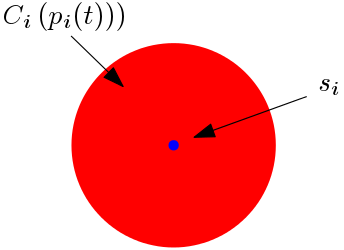
\includegraphics[scale=0.6]{figures/problem-def/sensor-and-coverage.png}
\caption{A sensor and its coverage region.}% \textcolor{red}{(you never reference the figure in text)}}
\label{fig:coverage region exmaple}
\end{figure}

%\subsection{Configuration}
A configuration $c$ of the mobile sensors at time $t$ is the stack of the sensor positions at time $t$,
\begin{equation}
c\left(t\right) = \bmat{
p_{1}^{T}\left(t\right)&\cdots&p_{n}^{T}\left(t\right)}^{T}\in\mathbb{R}^{2n}.
\label{eq:configuration definition}
\end{equation}
%\textcolor{red}{(all equations must have punctuation at the end (period, comma, semicolon, etc)}
Thus the coverage of a configuration is given by
\begin{equation*}
D\left( c\left( t \right) \right) = \cup C_i(p_i(t)).
\end{equation*}
%\textcolor{red}{(is the coverage $\cap C_i(p_i(t))$ or $\cup C_i(p_i(t))$?)}
We also emphasize in this work that we assume it is not possible to cover the entire area $A$ using a single configuration.
\begin{assumption}
For any configuration $c(t)$, the coverage satisfies $D\left( c\left( t \right) \right) \subset A$. % - a single configuration \emph{can't} provide full coverage!
\label{assump: no full coverage}
\end{assumption}

%\textcolor{red}{(missing a sentence that sets this up)}
We also introduce in this work a designated sub-area of the area $A$ that must remain under constant coverage.  In this direction, let us consider a sub-area of $A,\; A_m \subset A$. The area $A_m$ can represent a ground station communication constraint, a surveillance constraint etc., that means that $A_m$ must be partially covered at all times.
%\textcolor{red}{(please use text to introduce the assumption...explain what is going on then formally provide the assumption.}


\begin{figure}[H]
\centering
	\begin{subfigure}[b]{0.3\textwidth}
		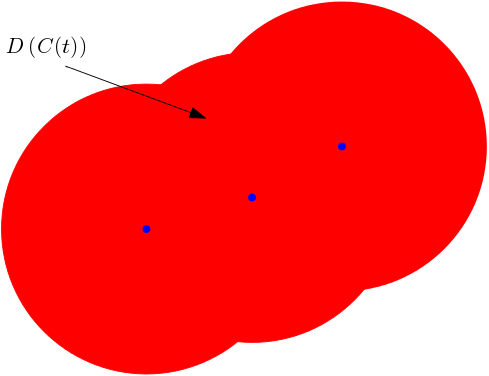
\includegraphics[width=\textwidth]{figures/problem-def/config-1.png}
	\end{subfigure}
	\hspace{0.75cm}
	\vline
	\hspace{0.75cm}
	\begin{subfigure}[b]{0.3\textwidth}
		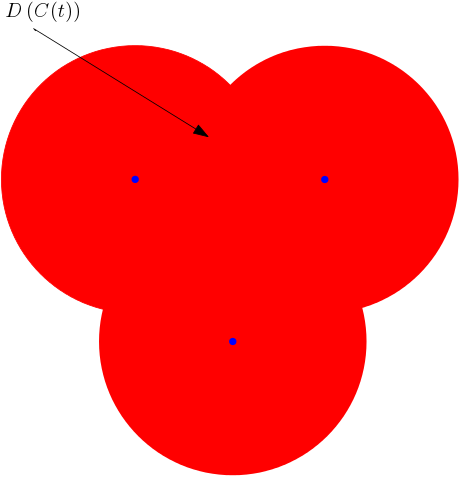
\includegraphics[width=\textwidth]{figures/problem-def/config-2.png}
	\end{subfigure}
	\caption{Two configurations built from the same sensors set.}
	\label{fig:configurations Example}
\end{figure}


%\subsection{Partition}
%\textcolor{red}{(please use more text to link together the pieces you are writing - tell a story)}

In Figure \ref{fig:configurations Example}, we can see how a given configuration can cover some area in different ways. However, due to Assumption \ref{assump: no full coverage} we know that it isn't possible using a single configuration. Therefore, we shall \emph{partition} the area, as can be seen in Figure \ref{fig:partition example}.

\begin{definition}
A \emph{partition} of $A \in \rsqr$, $PR(A)$ is a finite set built from $n$ subsets $pr_i \subset \rsqr,\; i=1,\; \ldots,\; n$ such that:
\begin{itemize}
\item $pr_i \cap pr_j = \emptyset \; \forall i \neq j$.
\item $\cup pr_i = A$.
\end{itemize}
\end{definition}

\begin{figure}[!ht]
\centering
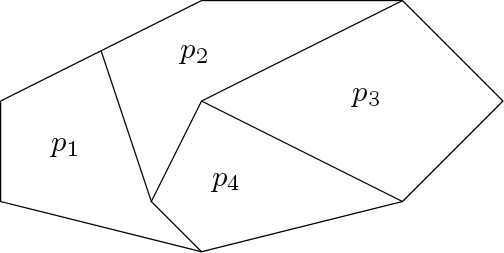
\includegraphics[scale=0.4]{figures/problem-def/partitioning.png}
\caption{An example of a partition of some area.}
\label{fig:partition example}
\end{figure}

This work aims to find a partition $PR(A)$ such that each of it's subsets $pr_i$ intersects with $A_m$, {and} that each $pr_i$ is eventually covered during the deployment.

\begin{problem} \label{GeneralProblem}

\begin{enumerate}[(a)] 
\item Find a partition $PR(A)$ such that each of the subsets $pr_i \in PR(A)$ satisfy $pr_i \cap A_m \neq \emptyset$;
\item Find a deployment controller for each sensor, such that $$ pr_i \subseteq \lim_{t\rightarrow \infty}D(c(t)),\text{for }i=1,\ldots,n.$$
\end{enumerate}
\end{problem}

In the following section, the basic mathematical concepts used in this work will be introduced, following by a solution for Problem \ref{GeneralProblem}. %\textcolor{red}{(what is Problem \ref{GeneralProbSolution}?)}
%\textcolor{red}{(use text to explain what the problem statement is! then say what you will discuss in next section to set things up)}

\section{Voronoi Diagrams and Distributed Coverage Algorithms}
%\textcolor{red}{(provide short paragraph summarizing what you will talk about here)}
In this chapter we will introduce two main concepts that were used in this work. The first is that of \emph{Voronoi diagrams}, and the later \emph{Lloyd's algorithm}.
\subsection{Voronoi Diagrams}
The basic mathematical concept that we employ in this work is the \emph{Voronoi Diagram} (also known as Voronoi partition or Voronoi tessellation). While being a method to partition an area with some cost function, it is a widely used in the optimal coverage problem \cite{Cortes2004,Hussein2007, Du1999}. 
%

The Voronoi Diagram of a region $\Omega \subset \rsqr$ is the set of partitions $\mathcal{V} = \left\{V_{1}, \ldots, V_n\right\}$ %\mid \cup V_{i} = \Omega\right\}$, 
generated by the generators $\mathcal{Z} = \{z_1,\ldots,z_n\mid z_{i} \in \Omega\}$, such that
\begin{equation} \label{Voronoi Definition}
V_{i} = \{q\in\Omega \mid \norm{q - z_i} \leq \norm{q - z_j} \forall z_i,z_j\in\mathcal{Z}\},
\end{equation}
and $\cup_i V_i = \Omega$, where %$V_{i}$ corresponds to the $i$-th element of $\mathcal{Z}$, and 
$\norm{\cdot}$ denotes the Euclidean distance.
%
A more intuitive and non-formal definition of the Voronoi Diagram is as follows. If we take some area and place points $p_i$ in it, then each partition is the set of all points that are closer to $p_i$ than $p_j$, when $j \neq i$. An example is the problem where there are post offices in some city, and it is needed to decide which house will be served by which specific post office. Using Voronoi partitioning, we can determine which houses are the nearest to each office and therefore conclude which houses each branch will serve. A visual example can be seen in Figure \ref{fig:Voronoi_tessellation_illustration}(a).
%\textcolor{red}{(you should already refer to your figure as an example)}
%\subsubsection*{Centroidal Voronoi Tessellation}

One can also define a density function, $\rho_i$, for each Voronoi partition $V_{i}$. Then, we can define the center of mass for each partition as,
\begin{equation}
z_{i}^{*} = \frac{\int_{V_{i}}y\rho(y)dy}{\int_{V_{i}}\rho(y)dy}.
\end{equation}
If a generator $z_{i} = z_{i}^{*} \, \forall \,V_{i}$, we call this partitioning a \emph{centroidal Voronoi tessellation} (CVT). Such tessellations are useful in terms of location optimization \cite{Cortes2004,Du1999,Atinc2013}.
A centroidal Voronoi tessellation illustration can be seen in Figure~\ref{fig:Voronoi_tessellation_illustration}(b). 

While Voroni diagrams are useful for partitioning some existing range, CVT is a technique used for (but not only) for \textit{planning} in an optimal way. If in the Voronoi diagram explanation, it was used to plan the delivery areas for each office, we will use the CVT to find where are the optimal locations to place the post offices.

\begin{figure}
	\captionsetup[subfigure]{position=b}
	\centering
	\subcaptionbox{Voronoi Diagram.}{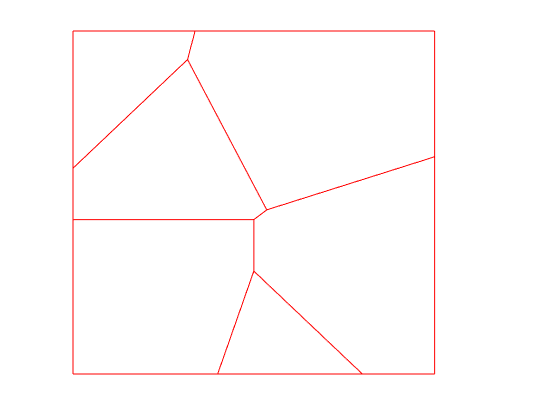
\includegraphics[width=.48\linewidth]{figures/math-bg/voronoi.png}}\label{fig:voronoi:voronoi}
	\subcaptionbox{Centroidal Voronoi Tessellations. The points represent the center of mass, calculated using the density function $\rho = 1$.}{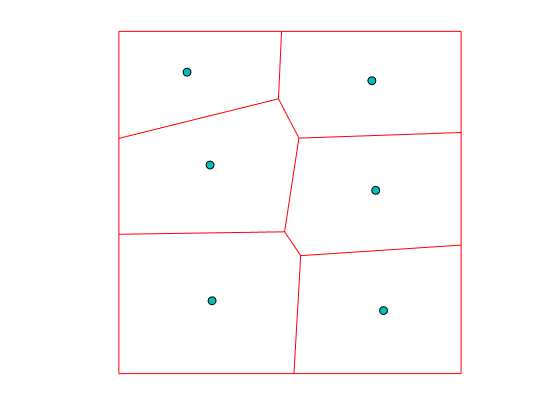
\includegraphics[width=.48\linewidth]{figures/math-bg/cvt.png}\label{fig:voronoi:cvt}}
	\caption{Illustration of Voronoi Diagram and a CVT, both from the same initial conditions}
\label{fig:Voronoi_tessellation_illustration}
\end{figure}

As can be seen in \eqref{Voronoi Definition}, the calculation of each Voronoi cell for some agent depends on the other agents positions. Therefore, any sort of calculation requires \emph{sharing information}. This can be done in a centralized approach (as it was done for this research), but there exists also decentralized calculations, for example \cite{Adams2009}. Using decentralized calculation, each agent only requires information from their neighbours (or any limited amount of agents). This allows calculating huge networks, in dynamic situations where the agents' network can be changed in real time.% \textcolor{red}{(run-on sentence! break up what you are saying into chunks)}.

\subsection{Lloyd's Algorithm}
As mentioned above, the CVT's are very useful for locational optimization. However, calculating the CVT might be a complicated task. Lloyd proposed a very simple way of calculating the CVT \cite{Lloyd1982}, presented in Alogirthm \ref{LloydAlgo}. 
\begin{algorithm}
\caption{Lloyd's Algorithm}\label{LloydAlgo}
\begin{algorithmic}[1]
\State Calculate the Voronoi diagram for the current agents positions.
\State Calculate the center of mass for every cell.
\State Move the agents to the center of mass.
\State Repeat until converge.
\end{algorithmic}
\label{algo:lloyd's algorithm}
\end{algorithm}

%\subsubsection*{Continuous-time Lloyd's Algorithm}
Cortes et al. \cite{Cortes2004} proposed a control algorithm based on Lloyd's algorithm.
Let us define a polygon $\mathcal{W} \subset \rsqr$. The basic deployment problem is finding a position $p \in \rsqr$ to maximize the coverage of the polygon $\mathcal{W}$. According to \cite{Cortes2004}, minimizing the function 
\begin{equation}
\mathcal{H}(p, \mathcal{W}) = \int_{\mathcal{W}} \norm{p-q}^2 dq
\label{eq:Lloyds optimization function}
\end{equation}
will yield the requested result.

The function $\mathcal{H}(p, \mathcal{W})$ measures the distance between a point $p$ to any point $q \in \mathcal{W}$. In \cite{Cortes2004}, this problem was expanded to the case of $n$ points, such that each point $p_i$ represent the $i$'th sensor position, and we are looking for the best partition $(\mathcal{W}_1, \ldots, \mathcal{W}_n)$ such that the coverage is maximized. Now, the total cost function will be:
\begin{equation}
\mathcal{H}(P, \mathcal{W}) = \sum_{i=1}^n \int_{\mathcal{W}} \norm{p_i-q}^2 dq.
\label{eq:vornoi cost function}
\end{equation}
The solution of this problem is the voronoi partition $\mathcal{V} = (V_1, \ldots, V_n)$.

The main challenge now is finding the points that maximize (\ref{eq:vornoi cost function}). According to \cite{Cortes2004}, when using Voronoi partitioning, (\ref{eq:vornoi cost function}) can be expressed as:
\begin{equation}
\mathcal{H}(P, \mathcal{V}) = \mathcal{H}_{\mathcal{V}}(P) = \int_{\Omega} \min_{i \in (1,\ldots, n)} \norm{p_i-q}^2 \phi(q) dq,
\label{eq:vornoi assumptions cost function}
\end{equation}
where $\phi(q)$ represents a measure of information or probability that some event take place over $\Omega$. For the rest of the problem, and for the sake of simplicity, we assume that $\phi(q) = \rho(q) = 1$.

It is possible to define the mass $M_{V_i}$ and the center of mass $C_{V_i}$ of the $i$'th Voronoi region:
\begin{align*}
M_{V_i} &= \int_{V_i} \rho(q)dq, \\
C_{V_i} &= \frac{1}{M_{V_i}} \int_{V_i} q\rho(q)dq.
\end{align*}
Cortes et al. \cite{Cortes2004} showed that at least one of the solutions for the optimization of (\ref{eq:vornoi assumptions cost function}) is the CVT:
\begin{equation}
C_{V_i} = \arg\min_{p_i} \mathcal{H}_{\mathcal{V}}(p).
\end{equation}

Assuming that a sensor has integrator dynamics, i.e., for each sensor, $\dot{p}_i = u_i$, \cite{Cortes2004} shows a way to implement Lloyd's algorithm as,
%
\begin{equation} \label{eq:Lloyds continuous time control}
u_{i} = -k_{prop}\left( p_i - C_{V_{i}} \right),
\end{equation} 
where $k_{prop}$ is a positive constant. Note that the dynamics in (\ref{eq:Lloyds continuous time control}), which minimizing (\ref{eq:Lloyds optimization function}), is a gradient dynamical system, and Cortes et al. \cite{Cortes2004} proved that the controller~(\ref{eq:Lloyds continuous time control}) is locally asymptotic stable.

%\textcolor{red}{(I think you should still mention the relation of above to gradient controllers)}

\section{Proposed Solution}

In this chapter, Problem \ref{GeneralProblem} will be addressed. First, we will propose an algorithm to address the special partition requirements, and then a solution for the whole problem will be shown.

\subsection{Projected Lloyd's Algorithm}
%\textcolor{red}{(please write more formally and make reference to our assumptions and problem statement - this is a bit too informal)} 
In this section, a solution for Problem \ref{GeneralProblem}(a) under Assumption \ref{assump: no full coverage} will be given. Recall that in Problem \ref{GeneralProblem}(a) it is required that for the partition of $A$, that $pr_i \cap A_m \neq \emptyset$ is satisfied.
%
To show the solution, we will first define a \emph{projection} onto the area $A_m$.
\begin{definition}
Consider a set $A_m \subset \mathbb{R}^2$ and a point $x \in \mathbb{R}^2$.  The \emph{projection} of $x$ onto $A_m$ is given by
$$\textsc{proj}_{A_m}(x) = \arg\min_{y \in A_m} \norm{x-y}^2.$$
\label{def:projection operator}
\end{definition}

Applying the projection operator in conjunction with Lloyd's algorithm yields the \emph{Projected Lloyd's Algorithm} (PLA), given in Algorithm \ref{ProjLloydsAlgorithm}. This combination allows solving Problem \ref{GeneralProblem}(a), and it is this work's main contribution.%\textcolor{red}{(be more explicit that this is your contribution!)}
\begin{algorithm}
\caption{Projected Lloyd's Algorithm}\label{ProjLloydsAlgorithm}
\begin{algorithmic}[1]
\State Calculate the Voronoi diagram for the current agents positions.
\State Calculate the center of mass for every cell.
\State Project the center of mass of every cell to the area constraint limiting polygon.
\State Move the agents the projected center of mass.
\State Repeat until converge.
\end{algorithmic}
\label{algo:PLA}
\end{algorithm}

As one can see, two more steps were added to the original Lloyd's algorithm - where we project the cell center of mass to the polygon that defines the area constraint (steps number 3-4), and then moving the agents to those points. Those step allows us to ensure that at least one agent will be \emph{on} the limiting polygon, thus we will have coverage within the constraint.

%\textcolor{red}{(you should refer explicitly to figure and explain what it is...)}
%\textcolor{red}{(I feel a lot of detail is missing here...)}
\begin{figure}
	\captionsetup[subfigure]{position=b}
	\centering
	\subcaptionbox{CVT calculated using Lloyd's algorithm}{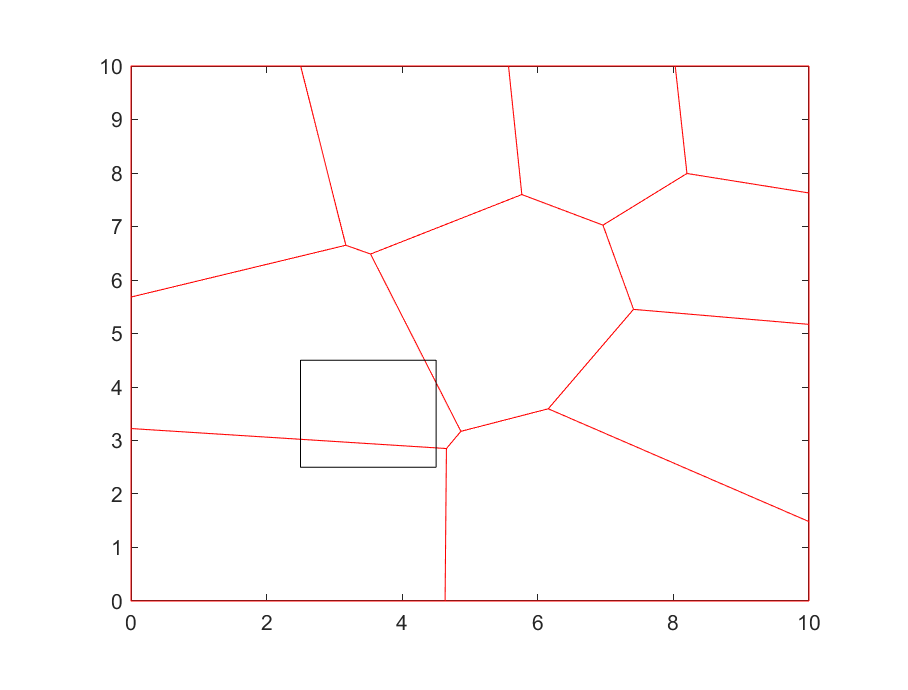
\includegraphics[width=.48\linewidth]{figures/proposed-sol/proj-lloyds-off.eps}}
	\subcaptionbox{PLA solution}{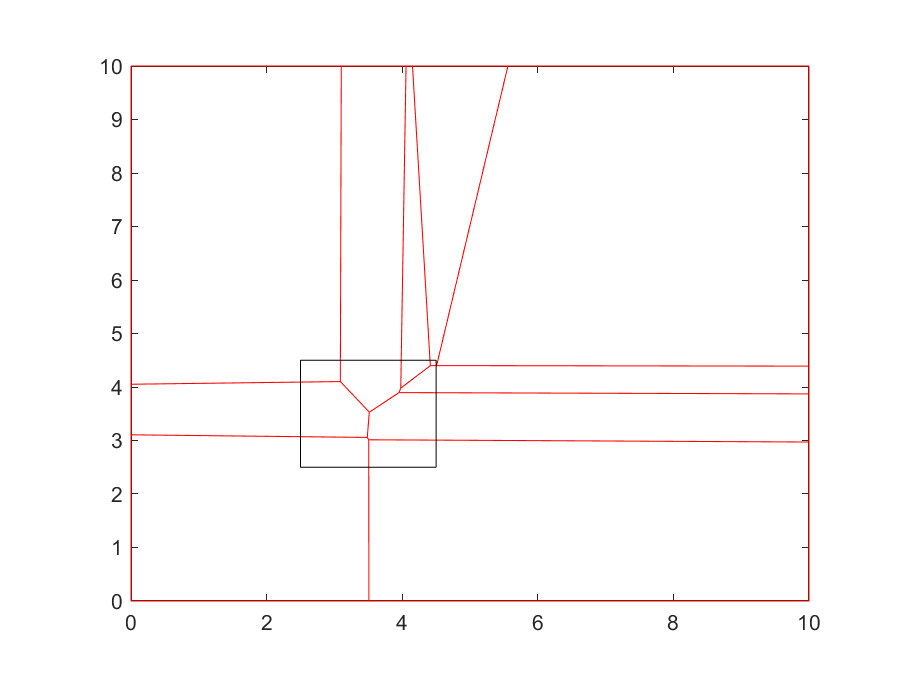
\includegraphics[width=.48\linewidth]{figures/proposed-sol/proj-lloyds-on.eps}}
	\caption{CVT and PLA solutions for initial conditions. The black box represents $A_m$.}
\label{fig:projected lloyds algorithm}
\end{figure}

In Figure \ref{fig:projected lloyds algorithm}, the PLA results can be clearly seen. For the same initial condition, Figure \ref{fig:projected lloyds algorithm}(a), it can be clearly seen that only 3 (out of 10 tiles) intersects with $A_m$. In Figure \ref{fig:projected lloyds algorithm}(b), the PLA algorithm was activated and all tiles intersect with $A_m$.

This algorithm can be also formed in a continuous time form, based on (\ref{LloydAlgo}), %\textcolor{red}{(please make sure notation is consistent!)}
\begin{equation} \label{ProjectedLloydsContol}
u_{i} = -k_{prop}\left( p_i - \textsc{proj}_{A_m}\left( C_{V_{i}} \right) \right).
\end{equation}
This continuous time controller, which is a modification of the controller proposed in \cite{Cortes2004}, is always converging into a solution where each tile intersects with $A_m$.

%\subsubsection*{Stability of the Projected Lloyd's Algorithm}
%\textcolor{red}{(text to setup theorem)}
In \cite{Cortes2004}, it was proven that the controller (\ref{eq:Lloyds continuous time control}) converges asymptotically to a set of critical points. It was done using (\ref{eq:vornoi assumptions cost function}) as a Lyapunov candidate function, and then, using La'Salle's invariance principal, it was shown that the sensors converged into $C_{V_i}$.  We employ this same idea to show the convergence of the projected Lloyd's algorithm.
\begin{theorem}
The controller proposed in (\ref{ProjectedLloydsContol}) is locally asymptotic stable.
\end{theorem}

%\textcolor{red}{please start by summarizing proof of Lloyd without projection}
\begin{proof}
Let us define a Voronoi partition moment of inertia:
\begin{equation}
J_{V,p} = \int_V \norm{q-p}^2 \rho(q)dq
\end{equation}
In \cite{Cortes2004} it was shown that:
\begin{align*}
\mathcal{H}_{\mathcal{V}}(P) &= \sum_{i=1}^n J_{V_i,C_{V_i}} + \sum_{i=1}^n M_{V_i} \norm{p_i - C_{V_i}}^2\\
\frac{\partial \mathcal{H}_{\mathcal{V}}}{\partial p_i} &= 2M_{V_i}\left( p_i - C_{V_i} \right).
\end{align*}
Let us define $\Psi(C_v, A_m) = \textsc{proj}_{A_m}\left( C_{V_{i}} \right)$. We must notice that $C_{V_i}$ is calculated in advance for each iteration, and therefore it is known.

Let us propose a candidate Lyapunov function:
\begin{equation}
\mathcal{\mathcal{H}_{\mathcal{P}}}(P) = \sum_{i=1}^n J_{V_i,C_{V_i}} + \sum_{i=1}^n M_{V_i} \norm{p_i - \Psi(C_v, A_m)}^2,
\end{equation}
it follows that \cite{Cortes2004}:
\begin{equation}
\frac{\partial \mathcal{H}_{\mathcal{P}}}{\partial p_i} = 2M_{V_i}\left( p_i - \Psi(C_v, A_m) \right).
\end{equation}
According to Lyapunov direct method, to prove asymptotic stability, one must show that
    \begin{itemize}
        \item[(1)] $\mathcal{\mathcal{H}_{\mathcal{P}}}(0) = 0$,
        \item[(2)] $\mathcal{\mathcal{H}_{\mathcal{P}}}(\zeta) > 0 \Leftrightarrow \zeta \neq 0$,
        \item[(3)] $\dot{{\mathcal{H}}}_{\mathcal{P}}(\zeta) < 0 \Leftrightarrow \zeta \neq 0$.
    \end{itemize}
Conditions 1,2 are direct from the definition of  $\dot{\mathcal{\mathcal{H}}}_{\mathcal{P}}(P)$.
As for condition 3, it is possible to see \cite{Cortes2004}:
\begin{equation*}
\frac{\partial \mathcal{H}_{\mathcal{P}}}{\partial p_i} = -2k_{prop} \sum_{i=1}^n M_{V_i} \norm{p_i - \Psi(C_v, A_m)}^2 < 0.
\end{equation*}
\end{proof}
%\textcolor{red}{(the key idea you must mention at beginning of the proof is that the point $C_{V_i}$ is somehow known/given/calculated \emph{a priori}, and thus so is its projection onto $A_m$...this makes the proof follow the same steps)}

Note that both the PLA and Lloyd's algorithm converge to some local minima of the cost function.  Lloyd's algorithm will converge to the CVT, but the PLA converges to some other tessellation determined by the projection onto the designated area $A_m$.
% \textcolor{red}{(it still converges to a local minimum!  its just now a different one)}
%\textcolor{red}{(Lloyd is not really optimial since in only can guarantee convergence to a local minima! The point is that Lloyd gives us a CVT while ours gives us some different partition)}


\subsection{Full Problem Solution Algorithm}
The PLA is answering the question of how to partition such that $pr_i \cap A_m \neq \emptyset$. The second part of the problem, which requires a deployment controller, was answered in \cite{Cortes2004}. It is possible to utilized their solution, proposing a solution algorithm for Problem \ref{GeneralProblem}.

\begin{algorithm}[H]
\caption{Problem \ref{GeneralProblem} Solution Algorithm}\label{GeneralProbSolution}
\begin{algorithmic}[1]
\State Using some random initial guess, calculate the PLA for the whole area.
\State For each partition (assuming that the agents can actually cover each partition with their coverage radius), calculate the CVT. The initial positions for the CVT calculation is the previous partition CVT.
\end{algorithmic}
\label{algo:problem solution algorithm}
\end{algorithm}

The above \emph{centralized} algorithm propose a simple method to solve Problem \ref{GeneralProblem}. Starting by partitioning the area while maintaining $pr_i \cap A_m \neq \emptyset$, and then calculating the optimal deployment for each partition. Assuming that the sensors can cover each partition using this deployment, the problem is solved. 
We must notice that in stage 1, the number of the tiles of the PLA solution is decided by the user (and does not take into account $D(c(t))$). Therefore, for the assumption in step 2 to hold, the user should wisely select the number of tiles, such that the agents can provide full coverage to each tile using the optimal deployment calculated in step 2.%\textcolor{red}{(I also do not follow the last two sentences - what is the point you are making here?)}
%\textcolor{red}{(I do not understand this sentence - you say the algorithm solves the problem and then you say it does not ensure that?)}
%As mentioned before, this algorithm is centralized and can be calculated a priori (at home base) or in real time, however it is \emph{centralized} - therefore for real-time calculations, some ground station or a single agent should perform the calculation and distribute the results to the agents.
% \textcolor{red}{(which calculation are you talking about?)}
%A note about the Voronoi diagram - The Voronoi diagram can be calculated even if the agents are outside of the required area. It does require sometimes more iterations. \textcolor{red}{(disjoint sentences like these are not good writing - you need to tie this into what you are saying..as it stands it just seems like a random comment)}

%\textcolor{red}{(I still think there needs to be more plain english explanation of what is going on)}
%\textcolor{red}{(this section needs more explaining...please see my mafat report as an example)}

\subsection{Results}
In this sub-section, we will show results for Problem \ref{GeneralProblem}, using Algorithm \ref{algo:problem solution algorithm}.
%
In the following simulations, the initial conditions were identical.

%\subsubsection{Results \emph{without} PLA}
\begin{figure}[H]
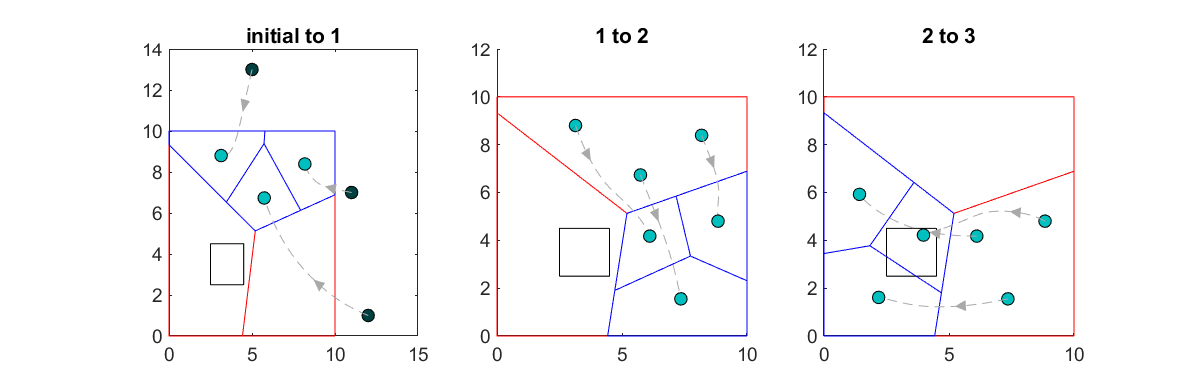
\includegraphics[scale=0.8]{figures/proposed-sol/results/sim1-3agents-3partitions-noPLA.eps}
\caption{Results without PLA. The box represents $A_m$.}
\label{fig:results no PLA}
\end{figure}

In Figure \ref{fig:results no PLA}, we can see a simulation for 3 agents. The area is partitioned into 3 tiles using Lloyd's algorithm (that is CVT), and each tile is covered using the algorithm proposed in \cite{Cortes2004}. The agents moved between the tiles in arbitrary order, and one can notice that only in the last step there was coverage of $A_m$.

%\subsubsection{Results \emph{with} PLA}
\begin{figure}[H]
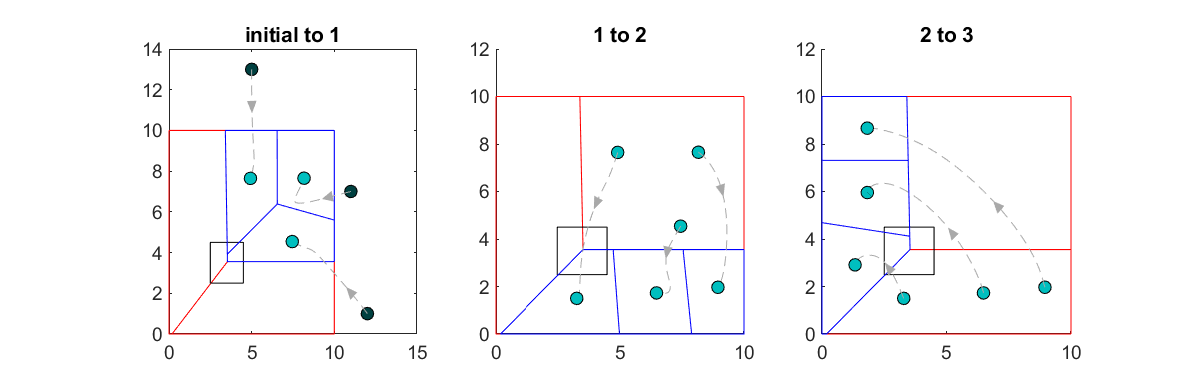
\includegraphics[scale=0.8]{figures/proposed-sol/results/sim2-3agents-3partitions-PLA.eps}
\caption{Results with PLA. The box represents $A_m$.}
\label{fig:results PLA}
\end{figure}

In Figure \ref{fig:results PLA}, we perform another simulation with 3 agents. The area is partitioned into 3 tiles using Projected Lloyd's algorithm, and each tile is covered using the algorithm proposed in \cite{Cortes2004}. The agents moved between the tiles in arbitrary order, and each tile has some partial coverage of $A_m$, as expected by the algorithm.

\section{Combining Lloyd's Algorithm and Distance-Based Formation Control}
Sometimes the agents topology should be constrained. For example, if the agent mission is search and rescue using geolocation calculation of emitters, then the spatial structure of the formation plays a major role in the system performance. We refer to this problem as the \emph{formation control} problem \cite{Oh2015}. In this chapter, the \emph{Distance-based} formation control will be combined with a deployment controller.%\textcolor{red}{(not a very convincing introduction to this section...)}

\subsection{Distance-Based Formation Control}
%\textcolor{red}{(I don't think you need all this background material on graphs and rigidity - simply write in one paragraph the tools used and appropriate references, then just present the controller (ie. your V.A.3 section).}
In this section, a short mathematical background will be given, following by this work contribution. 

\subsubsection{Mathematical Background}
A graph $\mathcal{G} = \left(V, \mathcal{E}\right)$ is a pair of two finite sets - the \emph{vertices} (nodes) set $V$ ($|V| = n$), and edges $\mathcal{E} \subseteq V\times V$. Each vertex can represent a mathematical or physical entity, for example - a sensor. Each edge represents some relation between two entities, for example - communication connectivity or congruent sensing range.
Given a configuration as defined in (\ref{eq:configuration definition}), we can define the \emph{connectivity graph} \cite{Muhammad2006}. A pair $\{\mathcal{G}, c\}$ mapping between a graph $\mathcal{G} = \left(V, \mathcal{E}\right)$ and a configuration $c$ is called a \emph{framework}. In \cite{Roth1979}, the properties of frameworks are defined, and the most important definition for this work is given - a \emph{minimally infinitesimally rigid framework} (MIR). In \cite{Muhammad2006} the formal definitions are given.\br
In brief, a framework is \emph{rigid} if every motion creates a new framework that maintains the connectivity graph $\mathcal{G}$ unchanged (in both terms of connections and distance between graph nodes). \emph{minimally rigid framework} is a rigid framework such that the removal of each edge in $\mathcal{G}$ will result in a non-rigid framework. A \emph{infinitesimally rigid framework} is a framework that maintains its rigidity for each infinitesimal movement of the framework nodes. A framework is MIR if it is infinitesimally rigid and minimally rigid.% \textcolor{red}{(but you did not give the definition in this work!)}.

A useful mathematical tool in this regard is the \emph{rigidity matrix} (complete definition can be found on \cite{Krick2008}). For this work, it will be marked as $R(c) \in \mathbb{R}^{|\mathcal{E}| \times 2|\mathcal{V}|}$. For example, \emph{a framework is infinitesimally rigid if and only if $\mathbf{rk}\left[R\right] = 2|\mathcal{V} | -3 = |\mathcal{E}|$} \cite{Tay1984}. As a result, MIR frameworks have full row rank.
%\textcolor{red}{(you need to provide, in basic words, a definition of what rigidity means, and then emphasize it can be checked using the rigidity matrix via a rank condition, and point the reader to relevant references for more detail)}

\begin{comment}
\subsubsection{Algebraic Graph Theory}
A graph $\mathcal{G} = \left(V, \mathcal{E}\right)$ is a pair of two finite sets - the \emph{vertices} (nodes) set $V$ ($|V| = n$), and edges $\mathcal{E} \subseteq V\times V$. Each vertex can represent a mathematical or physical entity, for example - a sensor. Each edge represents some relation between two entities, for example - communication connectivity or congruent sensing range. An edge connecting nodes $v_i, v_j$ is denoted $e_{ij} = \left\{v_i, v_j\right\}$. An \emph{undirected graph} is a type of graph where $\forall v_i, v_j \in V$ there exist both $e_{ij}$ and $e_{ji}$. A vertex degree (for an undirected graph) is the number of edges connected to it, and marked for vertex $i$ as $d_{i}$. 

The \emph{adjacency matrix} of a graph $\mathcal{G} = \left(V, \mathcal{E}\right), \; A(\mathcal{G})$ is a symmetric matrix such that $A(i,j) = 1$ if $\{v_i, v_j\} \in \mathcal{E}$ and $0$ otherwise.

The \emph{incidence matrix} of a graph $\mathcal{G} = \left(V, \mathcal{E}\right), \; E(\mathcal{G}))$ is a matrix such that $E(i,j) = 1$ when a node $v_i \in \mathcal{V}$ is incident to the edge $e_{ij} \in \mathcal{E}$, and $0$ otherwise.

\subsubsection{Graph Connectivity and Rigidity}
Given a configuration as defined in (\ref{eq:configuration definition}), we can define the \emph{connectivity graph} \cite{Muhammad2006}. Given a connectivity radius $R$ (assuming all the agents are identical in terms of connectivity radius), we define the \emph{connectivity graph} of a configuration $c$ as $\mathcal{G}_c\left(c, R \right) = \left(\mathcal{V,E}\right)$ such that each node $v_{i}$ of the graph is mapped to an agent position $p_{i}$. This mapping defines the pair $\left\{\mathcal{G}, c \right\}$, also known as a \textit{framework}. Given two graph nodes $v_{i},v_{j}, i\neq j$, then $\left\{v_{i}, v_{j}\right\} \in \mathcal{E} \Leftrightarrow \norm{p_{i} - p_{j}} \leq R$.

For the following definitions, $S(\mathcal{V})$ is the mapping between some configuration to the graph nodes set $\mathcal{V}$, and $S(v_l)$ is a mapping for a specific node $l$. All of those definitions can be found also in \cite{Roth1979}.

\begin{definition}
Two frameworks $(\mathcal{G}, S_0), (\mathcal{G}, S_1)$ are \emph{equivalent} if $$\;\norm{S_0(v_i) - S_0(v_j)} = \norm{S_1(v_i) - S_1(v_j)} \; \forall \; \{v_i, v_j\} \in \mathcal{E}$$\\
Two frameworks are \emph{congruent} if $$\;\norm{S_0(v_i) - S_0(v_j)} = \norm{S_1(v_i) - S_1(v_j)} \; \forall \; v_i, v_j \in \mathcal{V	}$$
\end{definition}

\begin{definition}
A framework $(\mathcal{G}, S_0)$ is rigid if there exists an $\epsilon > 0$ such that every framework $(\mathcal{G}, S_1)$ that is equivalent to $(\mathcal{G}, S_0)$ and satisfies $\norm{S_0(v) - S_1(v)} < \epsilon \; \forall \; v \in \mathcal{V}$,
is congruent to $(\mathcal{G}, S_0)$.
\end{definition}

\begin{definition}
A framework $(\mathcal{G}, S_0)$ is globally rigid if every framework that is equivalent to $(\mathcal{G}, S_0)$ is congruent to $(\mathcal{G}, S_0)$.
\end{definition}

\begin{definition}
A \emph{minimally rigid framework} is a rigid framework $(\mathcal{G}, S_0)$ such that
the removal of any edge in $\mathcal{G}$ results in a non-rigid framework.
\end{definition}

A complete definition the \emph{rigidity matrix} can be found in \cite{Krick2008}. For this work, it will be marked as $R(c) \in \mathbb{R}^{|\mathcal{E}| \times 2|\mathcal{V}}$.
\end{comment}

\subsubsection{Distance-Based Formation Controller}
Let us define a framework $\left\{\mathcal{G}, c \right\}$. The graph $\mathcal{G} = (\mathcal{V}, \mathcal{E})$ is a connectivity graph, and we also define the vector $D = \left[d_1, \ldots, d_{|\mathcal{E}|}\right]$ as the required length of each edge of the graph, while the actual length is given by $\norm{p_i-p_j}=\norm{e_k},\; e_k =(v_i,v_j) \in \mathcal{E}$. We can now define a \emph{formation potential} of a framework:
\begin{equation}
F(P) = \frac{1}{4}\sum_{k=1}^{\varepsilon}\left( \norm{e_k}^2 - d_{k}^{2} \right)^2 = \frac{1}{4}\sum_{k=1}^{\varepsilon} \sigma(p_i)_k^2 = \frac{1}{4}\sigma(P)^T \sigma(P),
\label{eq:formation potential}
\end{equation}
where $P$ is the positions vector of the agents in a configuration $c$, and $\sigma(P) = \left[\sigma_1, \ldots \sigma_\mathcal{E} \right], \; \sigma_{p_i} = \norm{e_i^2 - d_{i}^{2}}$.

A proposed controller is a gradient-dynamics based controller \cite{Kwang-KyoOh2011,Krick2008}:
\begin{equation}
\dot{p} = -\nabla F(p) = -R(p)^{T} R(p) p - R(p)^{T}D^2,
\label{eq:distance formation controller}
\end{equation}
where $D^2 = \left[d_1^2, \ldots, d_{|\mathcal{E}|}^2\right]$%\textcolor{red}{(you defined $D$ already above - but as a set and not a vector - please correct)}. %The controller is also related to the rigidity matrix!\\
The controller can be also defined for each individual agent. If $d_{ij}$ is the required distance between agents $i,j$ (that is the required distance assigned to the edge $e_k = \{v_i, v_j\}$), then
\begin{equation}
    \dot{p_{i}} = -\sum_{i \sim j} \left( \norm{p_{i} - p_{j}}^{2} - d_{ij}^2 \right) \left( p_{i} - p_{j} \right).
    \label{eq:distance formation controller for individual agent}
\end{equation}
Being a gradient dynamical system, it can be shown that this controller is locally asymptomatic stable if it has full row rank (that is, the framework is MIR) \cite{Kwang-KyoOh2011,Krick2008}.

\subsection{Combining Distance-Based Formation Control and Lloyd's Algorithm}
In this section, a combined deployment and formation controller will be shown. As both (\ref{eq:Lloyds continuous time control}) and (\ref{eq:distance formation controller}) are locally asymptomatic stable gradient descent controllers, it might be possible to combine them. Let us define a coefficient $0 \leq \alpha \leq 1$. The proposed controller for each agent is then
\begin{equation}
    u_{i} = \dot{p_{i}} = \alpha \left(-k_{p}\left( p_i -C_{V_{i}} \right)\right) +
    \left( 1-\alpha \right)\left[-\sum_{i \sim j} \left( \norm{p_{i} - p_{j}}^{2} - d_{ij}^2 \right) \left( p_{i} - p_{j} \right)  \right].
    \label{eq:Combined Controller}
\end{equation}
There are few interesting results regarding this controller.

\begin{proposition}
    Let us assume that there exists a Central Voronoi Tessellation (CVT), with $C_{V_{i}}$ such that $\forall i \neq j, \norm{C_{V_{i}} - C_{V_{j}}}^{2} = d_{ij}^{2}$ (that is $C_{V_{i}}$ satisfy the formation controller constraint). Then, there exists an equilibrium such that $P_e = C_V$ (where $P_{e_i} = C_{V_{i}}$ and $C_V = \left[C_{V_1}, \ldots, C_{V_n} \right]$), which is locally asymptotic stable with (\ref{eq:Combined Controller}) dynamics.
    \label{proposition 1}
\end{proposition}

\begin{proof}
    First of all, let us show that $P_e = C_{V}$ is an equilibrium point of \eqref{eq:Combined Controller}.  Indeed, by assumption, we have $\forall i \neq j, \norm{C_{V_{i}} - C_{V_{j}}}^{2} = d_{ij}^{2}$, so $\norm{p_{e_i} - p_{e_j}}^{2} = \norm{C_{V_{i}} - C_{V_{j}}}^{2} =d_{ij}^{2}$, showing $P_e = C_{V}$ is an equilibrium point. \br

    Now we are ready to prove that this equilibrium is stable. Let us choose a candidate Lyapunov function for the combined controller, which is a combination of the Lyapunov functions for each controller \cite{Cortes2004}: %\textcolor{red}{(what is the notation $\sigma(P)$ and $\sigma^t(P)$? be consistent and try not to introduce new notations for things already defined earlier)}
    \begin{equation}
        V_{c}\left(P\right) = \alpha\left[ \sum_{i=1}^{n} \int_{V_{i}} \min_{i\in \left\{1,\ldots, n\right\}} \norm{q-p_{i}}^2\phi(q)dq \right] + (1-\alpha) \left[ \frac{1}{4}\sigma(P_e)^{T} \sigma(P_e) \right],
        \label{Proposition 1 Lyapunov function candidate}
    \end{equation}
    where $ J_{V_{i},C_{V_{i}}}, M_{V_{i}}$ are as defined in \cite{Cortes2004}. %\textcolor{red}{(so this $\sigma_i$ is different than the one introduced earlier? notation overload)}
%
    Since the equilibrium is $P_e = C_{V}$ , we will change the variables, so $\zeta = P_e - C_{V}$, hence:
    \begin{equation}
        V_{c}\left(\zeta\right) = \alpha\left[ \sum_{i=1}^{n} \int_{V_{i}}\min_{i\in \left\{1,\ldots, n\right\}} \norm{q-\zeta_{i} - C_{V_{i}}}^2 \phi(q) dq\right] + (1-\alpha) \left[ \frac{1}{4}\sigma ^{T} (\zeta + C_{V_{i}})\sigma(\zeta + C_{V_{i}}) \right].
    \end{equation}
    According to Lyapunov direct method, to prove asymptotical stability, one have to show:
    \begin{itemize}
        \item[(1)] $V_{C}(0) = 0$,
        \item[(2)] $V_{C}(\zeta) > 0 \Leftrightarrow \zeta \neq 0$,
        \item[(3)] $\dot{V}_{C}(\zeta) < 0$.
    \end{itemize}
For condition (1) \cite{Cortes2004}, $$V_{C}(0) = \alpha\left[ \sum_{i=1}^{n} \int_{V_{i}}\min_{i\in \left\{1,\ldots, n\right\}} \norm{q- C_{V_{i}}}^2 \phi(q) dq\right] + (1-\alpha) \left[ \frac{1}{4}\sigma ^{T} (C_{V_{i}})\sigma(C_{V_{i}}) \right] .$$ 
    While it is obvious that $\sigma(C_{V_{i}}) = 0$, we have to look into the first term of the Lyapunov function. It is obvious that there is a minimum at $C_{V}$, therefore the integral gets him minimal value over there. Moreover, since the function we are minimizing is for the form $f(x) = x^{2}$, the minimum is $0$. Therefore, condition $(1)$ applies. 
    
For condition (2), it's obvious that both terms are strictly positive for $\zeta \neq 0$.
For condition (3), the combined derivative of the combined Lyapunov function is \cite{Cortes2004}:
    \begin{equation}
        \dot{V}_{C}(\zeta) = \alpha \left[ -2k_{p}\sum_{i=1}^{n}M_{V_{i}}\norm{p_{e_{i}} - C_{V_{i}}}^{2} \right] + (1-\alpha)\left[ -\sigma(P_e)^{T}R(P_e)R^{T}(P_e)\sigma(P_e) \right] \leq 0.
    \end{equation}
    As we can see, this term is smaller \emph{or equal} to zero. Therefore, using Lyapunov method, this system is stable, however not asymptotically stable. That said, we can notice that the set $S = \left\{ P = C_{V} \right\}$ doesn't contain any trajectory apart from the trivial trajectory (when $\zeta = 0$), therefore by LaSalle principal, the system is Locally asymptotic stable.
\end{proof}

\begin{theorem}
The dynamic system described by the controller (\ref{eq:Combined Controller}) asymptotically converges to a critical point of the function $G(p) = \alpha \mathcal{H}_{\mathcal{V}}(p) + (1-\alpha) F(p)$, where $F(p)$ is the distance-based formation controller (\ref{eq:distance formation controller})  potential, and $\mathcal{H}_{\mathcal{V}}(p)$ is the Voronoi-based deployment controller (\ref{eq:Lloyds continuous time control}) potential function\cite{Cortes2004}.
    \label{theorem: combined controller stability}
\end{theorem}
\begin{proof}
Both the formation control and the deployment controller can be expressed as a gradient dynamics system. It is
known that gradient flows converge to the critical points of the potential function.
\end{proof}

%\subsection{The Combination and Problem \ref{GeneralProblem}}

\begin{remark}As the combination of controllers provide some interesting results, it is very important to remember that it doesn't necessarily solves Problem \ref{GeneralProblem}. The reason is that the formation is changing the deployment, thus the condition for full area coverage might be broken. This work \emph{does not} provide a condition where the formation control holds \emph{and} Problem \ref{GeneralProblem} is fully solved.
\end{remark}
\subsection{Simulations}

\begin{figure}[H]
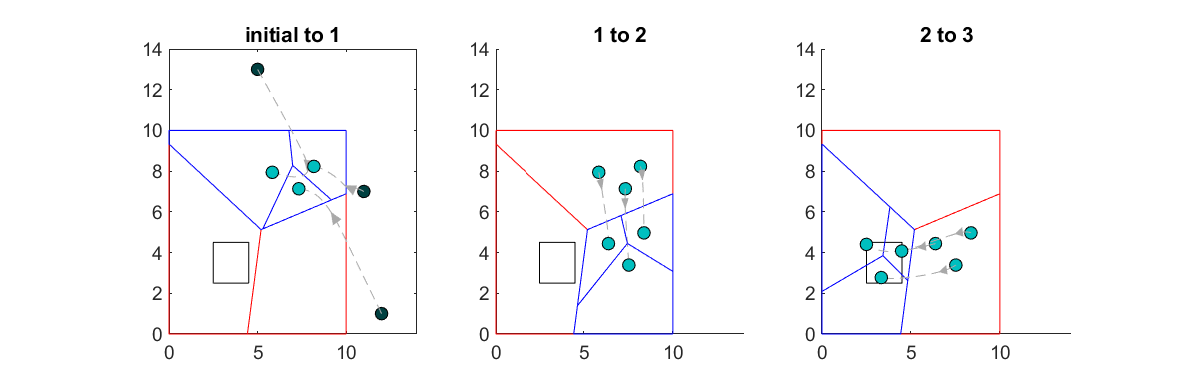
\includegraphics[scale=0.8]{figures/proposed-sol/results/sim3-3agents-3partitions-noPLA-formation.eps}
\caption{Results of the combination of Lloyd's algorithm and distance-based formation controller. The black box represents $A_m$.}
\label{fig:results formation, no PLA}
\end{figure}

In Figure \ref{fig:results formation, no PLA}, we can see a simulation for 3 agents where a triangular formation was defined ($d_{12} = d_{13} = 1,\; d_{23} = 2$), and combined with Lloyd's algorithm, with $\alpha = 0.5$. Comparing to Figure \ref{fig:results no PLA}, which can be seen as the same simulation where $\alpha = 1$, it is clear that the agents are having a more triangular shape.

\begin{figure}[H]
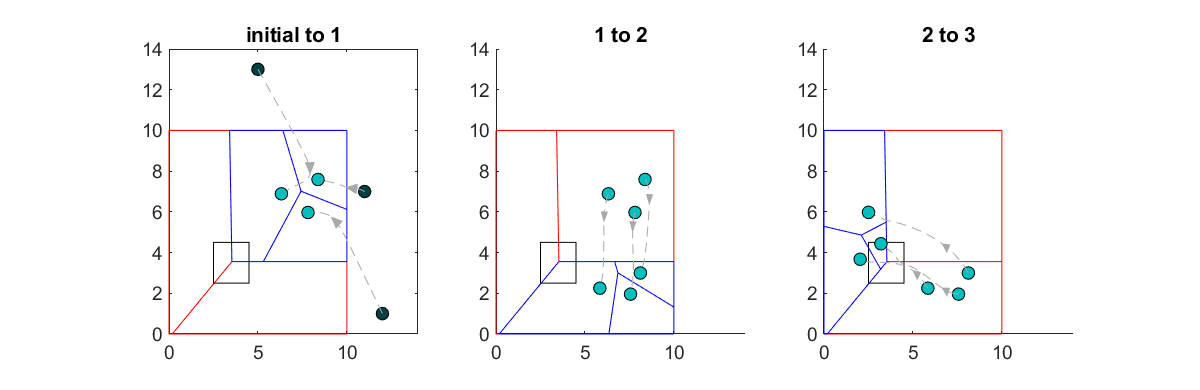
\includegraphics[scale=0.8]{figures/proposed-sol/results/sim4-3agents-3partitions-PLA-formation.eps}
\caption{Results of the combination of PLA and distance-based formation controller. The black box represents $A_m$.}
\label{fig:results formation, PLA}
\end{figure}

In Figure \ref{fig:results formation, PLA}, we can see a simulation for 3 agents where a triangular formation was defined ($d_{12} = d_{13} = 1,\; d_{23} = 2$), and this time combined with PLA, with $\alpha = 0.5$. Comparing to Figure \ref{fig:results PLA}, and similar to Figure \ref{fig:results formation, no PLA}, it is clear that the agents are having a more triangular shape.

%\textcolor{red}{(if you are not using the PLA, then it does not make sense to show the sub-area in the simulations.  Furthermore, you should either include a simulation with the PLA to show above works in both cases.)}

\section{Concluding Remarks}
The deployment problem under different constraints is a well known and researched problem. This work provides a new approach for partial coverage problem. When some sub-range should be covered constantly, this work presents a sequential coverage strategy, jumping between tiles. The Projected Lloyd's Algorithm, presented in this work, guarantees at least partial coverage of this sub range. Another contribution of this work is the combination of Lloyd's algorithm with a distance-based formation controller to achieve some spatial properties.

As the PLA is calculated in a centralized way, future work might include decentralizing its calculation. Future work might also include a condition for formation and deployment solution while maintaining some deployment and/or formation properties, as well as combining other types of formation controllers. Decentralizing the PLA, together with finding this condition, can lead to some interesting results for autonomous, dynamically changed swarms.

\bibliography{bibliography}
\bibliographystyle{iacas}
\end{document}
